\documentclass[a4paper]{paper}
\usepackage[utf8]{inputenc}
\usepackage[margin=2.5cm]{geometry}
\usepackage{enumitem}
\usepackage{float}
\usepackage[labelfont=bf,textfont=md]{caption}
\usepackage{graphicx}
\usepackage{xcolor}
\usepackage{minted}
\usepackage{hyperref}
\usepackage[all]{hypcap}
\usemintedstyle[common-lisp]{default}
\newmintinline[code]{text}{}
\bibliographystyle{plainnat}

\hypersetup{
  colorlinks,
  linkcolor={red!50!black},
  citecolor={blue!50!black},
  urlcolor={blue!80!black}
}

\newlist{step}{enumerate}{10}
\setlist[step]{label*=\arabic*.,leftmargin=2em}

\title{Using a Highly Dynamic Language for Development}
\subtitle{Advantages of and lessons learned from using Common Lisp in games}
\author{Nicolas Hafner}
\institution{Shirakumo Games}

\begin{document}
\twocolumn[\maketitle]

\begin{abstract}
  Games face an interesting challenge. They require rapid development, are highly interactive, and pose hard real-time performance constraints. While smaller games these days have also been developed in dynamic languages such as Python or Lua, traditionally engines are still written in static languages like C++ and C, with an additional scripting languages on top to handle gameplay mechanics. In this paper we explore using Common Lisp for full stack game development and outline the advantages this can bring to the development process, as well as the pitfalls and problem areas that are unique to this kind of approach.
\end{abstract}
\begin{keywords}
  Common Lisp, game development, dynamic languages, object orientation
\end{keywords}

\def\abovecaptionskip{1pt}
\def\listingautorefname{Listing}
\def\figureautorefname{Figure}

\section{Introduction}
Video games pose an interesting engineering challenge. They are highly dynamic in their nature, as users can perform various, sometimes far-reaching changes to the program at any time, and yet they must remain responsive under hard real-time constraints. Additionally, the development of games itself is highly dynamic, as changes to the game require constant testing and refinement. Long pauses between making a change and being able to properly evaluate its effects can gravely discourage testing, which leads to a much worse product.

A typical approach to solve this set of constraints is to use multiple languages in combination. A rather low-level language like C++ or C to handle the ``core engine'', and an integrated scripting language like Lua to handle gameplay logic. However, this approach has multiple issues of its own: it can be hard to distinguish which parts should be a part of the core engine, and which should not. The scripting cannot integrate with everything the engine offers, as an explicit interface has to be designed that can deal with the scripting language's own data types and routines. For performance reasons a highly dynamic part may also need to be lowered down into the static language, making iteration much slower and harder to deal with.

Finally, the lack of runtime debugging means that any problems appearing in the core engine often lead to a crash of the entire program, which makes diagnosing and fixing the issue much harder. This difficulty often leads to defensive programming strategies, where errors are simply ignored or otherwise coerced, leading them to cause issues further down the line, complicating debugging of the final product even more.

In this paper we instead take a holistic approach, using Common Lisp for the full stack of both the core engine and the gameplay tools and mechanics. Common Lisp is a highly dynamic language, allowing runtime redefinition of functions, variables, and classes, even to the point of completely reloading or changing an underlying library or system while the program is being executed. Yet, despite this dynamism, Common Lisp is a compiled language that takes great care to support the writing of efficient code. Highly optimising compilers like SBCL allow you to write fast code without having to drop down into another language.

We explore some of the aspects of Common Lisp that make it particularly suited for games in detail, and also discuss some of the pitfalls we encountered and how to combat them.

\section{Related Works}


\section{Modularity Through Mixins}
The Common Lisp Object System (CLOS) has a couple of traits that remain rare in programming languages in use today, but make for excellent tools to support game development. Relevant to this section are serialised multiple inheritance and the standard generic function method combination.

In CLOS methods are not attached to classes, but are instead parts of a generic function. Methods ``specialise'' on one or several of the required arguments of the function to a class. When the generic function is called, the system must first determine the set of ``applicable methods''. This set depends on the method combination used by the generic function. For brevity's sake, we will only look at the standard method combination here.

The standard method combination offers methods in four flavours: \code{primary}, \code{:before}, \code{:after}, and \code{:around}. These methods are grouped together, then filtered for applicable methods by checking whether the arguments passed to the generic function match their specialised classes, and finally sorted by \textit{how} specific the specialisations are to the arguments passed. With this completed set, the methods are invoked as illustrated in \autoref{fig:method combination}.

\begin{figure}[h]
  \centering
  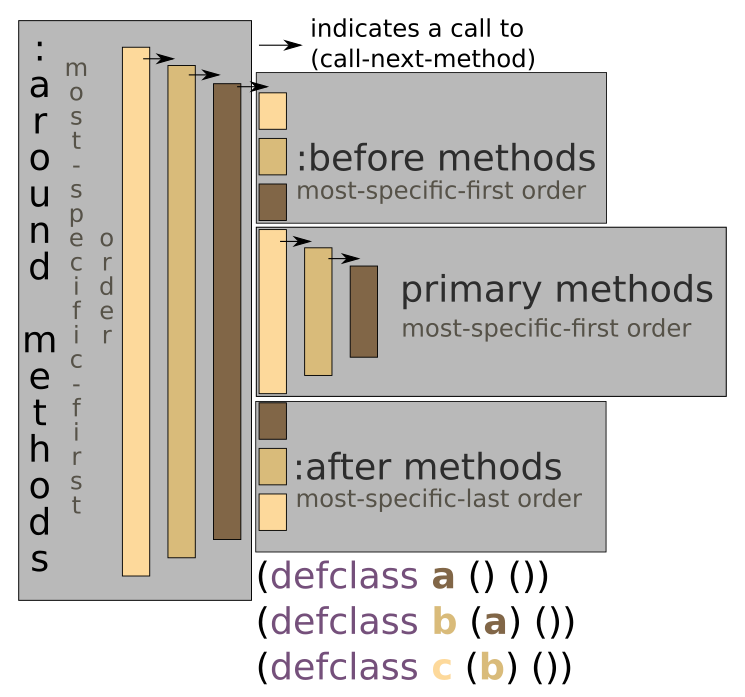
\includegraphics[width=0.4\textwidth]{method combination.png}
  \caption{The standard method combination behaviour illustrated}
  \label{fig:method combination}
\end{figure}

As a brief example, let us consider \autoref{lst:method definition}. Here we define a generic function of two arguments called \code{handle}, as well as three methods. All of the methods require the first argument to be a subclass of \code{tick}. Method 1 and 2 also require the second argument to be a subclass of \code{player}, and method 3 a subclass of \code{enemy}.

\begin{listing}[h]
\begin{minted}[fontsize=\scriptsize]{common-lisp}
(defgeneric handle (event object))

(defmethod handle         ((ev tick) (object player))) ; 1
(defmethod handle :before ((ev tick) (object player))) ; 2
(defmethod handle         ((ev tick) (object enemy)))  ; 3
\end{minted}
\caption{A brief example of method definition}
\label{lst:method definition}
\end{listing}

\hypertarget{first-call}{When \code{handle} is now called with a \code{tick} and a \code{player} instance, first the method 2 is executed, followed by the method 1. Method 3 is ignored, as it does not match the arguments.}

This method combination mechanism only really shines once we consider inheritance and especially multiple inheritance and the arising ``mixin classes''. Let us now define the classes we used for the previous listing. \autoref{lst:inheritance} shows five classes being defined, with \code{tick} being a subclass of \code{event}, and \code{player} and \code{enemy} being subclasses of \\\code{physics-object}.

\begin{listing}[H]
\begin{minted}[fontsize=\scriptsize]{common-lisp}
(defclass event () ())
(defclass tick (event) ())

(defclass physics-object () ())
(defclass player (physics-object) ())
(defclass enemy (physics-object) ())
\end{minted}
\caption{A brief example of method definition}
\label{lst:inheritance}
\end{listing}

We'll now also change the second method to specialise on the \code{physics-object} instead of \code{player}. For example, since both \code{player} and \code{enemy} are moving, we could be handling the collision resolution there. If we now perform the \hyperlink{first-call}{same call from before}, Methods 2 and 1 will still be invoked. However, unlike before, if we call the function with \code{tick} and \code{enemy}, now methods 2 and 3 will be invoked, instead of only method 3.

\begin{listing}[h]
\begin{minted}[fontsize=\scriptsize]{common-lisp}
(defmethod handle :before ((ev tick) (object moving-entity)))
\end{minted}
\caption{The updated second method definition}
\label{lst:updated method}
\end{listing}

In other OOP paradigms a similar behaviour can usually be achieved by calling the superclass' method with \code{super}, but notice here that the behaviour of method 2 does not require changing anything about the other methods or subclasses. It thus remains wholly encapsulated in its own behaviour.

So far so good. Now imagine that we decide enemies, should emit a light so that they're always visible. To implement this, we're going to define a new class, \code{emitter}, and define the light flicker behaviour in a new \code{handle} method as shown in \autoref{lst:emitter}.

\begin{listing}[h]
\begin{minted}[fontsize=\scriptsize]{common-lisp}
(defclass emitter () ())

(defmethod handle :before ((ev tick) (object emitter)))
\end{minted}
\caption{The new class and method to handle light flickering}
\label{lst:emitter}
\end{listing}

To make the enemy adopt this new behaviour, all we need to do is add \code{emitter} to the \code{enemy} class' superclass list. Thanks to the method combination, calls to \code{handle} will now include the \code{emitter}'s method, and we have achieved the combination of the two behaviours.

\begin{listing}[H]
\begin{minted}[fontsize=\scriptsize]{common-lisp}
(defclass enemy (physics-object emitter) ())
\end{minted}
\caption{The updated enemy class definition}
\label{lst:new-enemy}
\end{listing}

The order of the superclasses here is important. Classes that appear earlier in the list have ``precedence'' and are thus considered to be ``more specific'' when determining the set of applicable methods. By having \code{emitter} appear after \code{physics-object}, we ensure that the \code{emitter}'s \code{:before} method runs \textit{after} that of \code{physics-object}, ensuring the collisions have already resolved properly once we consider the lighting update.

Not having the \code{emitter} be a subclass of \\\code{physics-object} ensures that we can also use it as a superclass for other things such as completely static lanterns that have no business having any interactivity.

As an example from our actual code base, as of writing, the \code{player} class has 8 direct superclasses whose behaviours are combined together with the \code{player}'s own. This combination of behaviours allows encapsulating different parts and re-using them in many cases. Keep in mind, too, that all of these classes and methods can be redefined at runtime to change, add, and remove behaviours from an object while the game is still running.

However, one issue that crops up when segregating behaviours into such small compartments is that you might not have enough control over the combination of them. The standard method combination offers no fine-grained control to exclude or reorder methods for a specific specialisation of an argument. One could devise their own method combination strategy to allow this kind of specialised behaviour, however we are not convinced that this would not lead to an ultimately even more confusing design.

While the standard method combination and mixins offer a great deal of flexibility out of the gate, great care must still be taken when designing the overall class hierarchy and function protocol. Otherwise behaviours will not combine cleanly and lead to strange bugs, or might not combine properly at all.

\section{Restarts}


\section{Optimisation}


\section{Garbage Collection}


\section{Conclusion}


\section{Acknowledgements}


\bibliography{paper}
\end{document}


%%% Local Variables:
%%% mode: latex
%%% TeX-command-extra-options: "-shell-escape"
%%% TeX-master: t
%%% TeX-engine: luatex
%%% End:
